% Fig. 1 of the Pattern Recognition manuscript: study design and analysis workflow.
% Redrawn in TikZ (no image-generation tool) after the Springer Fig. 1
% (paper/manuscript/figure1_workflow.pdf): same five panels, boxes, icons and
% wording, changed only where the three encoders require it (panel b encoders,
% <Encoder> in panels c and e, Benjamini-Hochberg per encoder).
% The three MRI slices are the ones embedded in the Springer figure, padded to squares
% with their black background (slice_*_square.png).
% Build: pdflatex figure1_workflow.tex  ->  ../figure1_workflow_3enc.pdf (copied by the caller)
\documentclass[tikz,border=1pt]{standalone}
\usepackage[T1]{fontenc}
\usepackage{helvet}
\renewcommand{\familydefault}{\sfdefault}
\renewcommand{\mddefault}{c}% Helvetica Narrow, as in the original figure
\renewcommand{\bfdefault}{bc}
\usepackage{graphicx}
\usepackage{fix-cm}
\usetikzlibrary{arrows.meta,calc,positioning,shadows,decorations.pathreplacing}

\definecolor{edge}{HTML}{4D545E}
\definecolor{ink}{HTML}{2B2F36}
\definecolor{muted}{HTML}{5F6670}
\definecolor{blueF}{HTML}{E8EEF7}
\definecolor{greenF}{HTML}{E7F1E0}
\definecolor{tealF}{HTML}{E1EFEC}
\definecolor{pinkF}{HTML}{F7DEDE}
\definecolor{yellowF}{HTML}{F5C451}
\definecolor{nodeG}{HTML}{CFE5C3}

\newcommand{\fs}{\fontsize{6.9}{7.7}\selectfont}
\newcommand{\fsm}{\fontsize{6.2}{6.9}\selectfont}
\newcommand{\enc}{$\langle$Encoder$\rangle$}

\tikzset{
  >={Stealth[length=4pt,width=3.4pt]},
  box/.style={rounded corners=2.4pt, draw=edge, line width=0.55pt, align=center,
              font=\fs, text=ink, inner sep=1.5pt,
              drop shadow={shadow xshift=0.35pt, shadow yshift=-0.45pt, opacity=0.16}},
  bluebox/.style={box, fill=blueF}, greenbox/.style={box, fill=greenF},
  tealbox/.style={box, fill=tealF}, pinkbox/.style={box, fill=pinkF},
  title/.style={font=\fontsize{7.9}{8.8}\selectfont\bfseries, text=ink, align=center, anchor=north},
  letter/.style={font=\fontsize{9.5}{10}\selectfont\bfseries, text=ink, anchor=north west, inner ysep=2.5pt},
  flow/.style={->, line width=0.7pt, draw=ink},
  thin/.style={line width=0.5pt, draw=ink},
  lab/.style={font=\fsm, text=ink, align=center},
}

% Icons ---------------------------------------------------------------
\newcommand{\scatter}[1]{% prediction scatter in a rounded square centred at #1
  \begin{scope}[shift={#1}]
    \draw[bluebox, drop shadow={opacity=0}, fill=white] (-0.25,-0.25) rectangle (0.25,0.25);
    \draw[thin, dashed, line width=0.4pt] (-0.17,-0.17) -- (0.17,0.17);
    \foreach \p in {(-0.12,-0.04),(-0.04,0.06),(0.03,-0.07),(0.1,0.12),(0.12,0.03),(-0.1,0.1)}
      \fill[ink] \p circle (0.022);
  \end{scope}}
\newcommand{\person}[1]{%
  \begin{scope}[shift={#1}]
    \draw[thin, line width=0.45pt] (0,0.13) circle (0.055);
    \draw[thin, line width=0.45pt] (-0.09,-0.05) arc (180:0:0.09 and 0.1);
  \end{scope}}
\newcommand{\cycle}[1]{%
  \begin{scope}[shift={#1}]
    \draw[thin, line width=0.55pt, ->, >={Stealth[length=2.6pt,width=2.4pt]}] (60:0.16) arc (60:390:0.16);
  \end{scope}}

\begin{document}
\begin{tikzpicture}[x=1cm, y=1cm]
\useasboundingbox (0,0.95) rectangle (18.88,7.43);

% ===================================================== a: cohort and imaging
\node[letter] at (0,7.4) {a};
\node[title] at (1.55,7.4) {Cohort and imaging};
\node[bluebox, minimum width=2.75cm, minimum height=0.72cm] at (1.55,6.0) {Longitudinal\\ADNI cohort};
\node[font=\fs, text=ink] at (1.55,5.05) {T1-weighted MRI};
\node[inner sep=0] at (1.55,4.25) {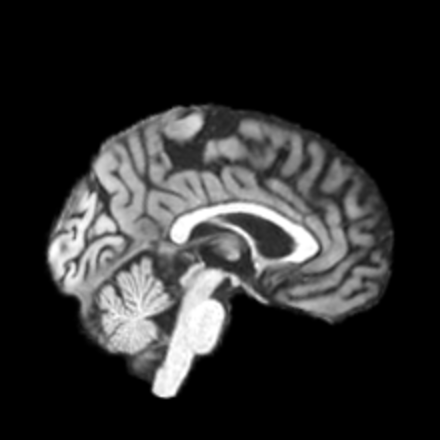
\includegraphics[width=0.92cm]{slice_sagittal_square.png}\hspace{0.6mm}%
  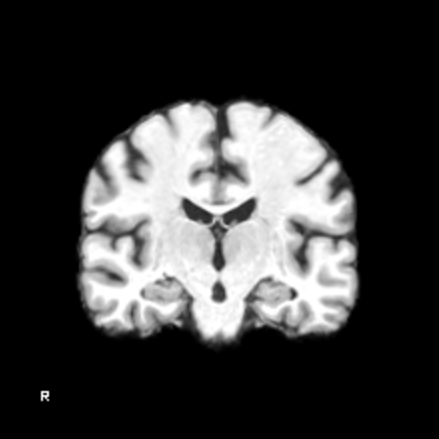
\includegraphics[width=0.92cm]{slice_coronal_square.png}\hspace{0.6mm}%
  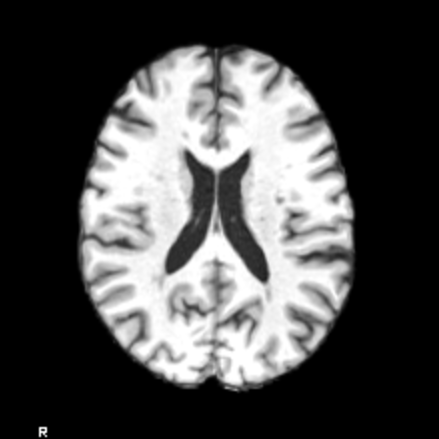
\includegraphics[width=0.92cm]{slice_axial_square.png}};
\node[bluebox, minimum width=2.75cm, minimum height=0.82cm] at (1.55,2.75) {};
\node[font=\fs, text=ink, align=center] at (1.79,2.75) {Eligibility and\\quality control};
\begin{scope}[shift={(0.69,2.75)}]% clipboard checklist
  \draw[thin, rounded corners=1pt, fill=white] (-0.16,-0.25) rectangle (0.16,0.22);
  \draw[thin, rounded corners=0.6pt, fill=white] (-0.06,0.19) rectangle (0.06,0.27);
  \foreach \y in {0.09,-0.03,-0.15} {
    \draw[thin, line width=0.4pt] (-0.11,\y-0.03) rectangle (-0.05,\y+0.03);
    \draw[thin, line width=0.45pt] (-0.01,\y) -- (0.11,\y);}
\end{scope}

\draw[flow] (3.2,4.25) -- (3.68,4.25);

% ===================================================== b: frozen encoders
\begin{scope}[xshift=0.22cm]
\node[letter] at (3.58,7.4) {b};
\node[title] at (5.15,7.4) {Foundation model\\representation};
\foreach \name/\y in {Neuro-JEPA/6.1, DINOv3/5.48, BrainIAC/4.86}
  \node[greenbox, minimum width=2.95cm, minimum height=0.5cm, font=\fontsize{7.1}{7.8}\selectfont\bfseries] at (5.15,\y) {\name};
\begin{scope}[shift={(5.15,3.95)}]% frozen network
  \foreach \x in {-0.62,0,0.62}
    \draw[thin, rounded corners=3pt, fill=white] (\x-0.1,-0.4) rectangle (\x+0.1,0.4);
  \foreach \ya in {0.27,0.09,-0.27} \foreach \yb in {0.27,0.09,-0.27} {
    \draw[thin, line width=0.3pt] (-0.62,\ya) -- (0,\yb); \draw[thin, line width=0.3pt] (0,\ya) -- (0.62,\yb);}
  \foreach \x/\f in {-0.62/white,0/nodeG,0.62/nodeG} {
    \foreach \y in {0.27,0.09,-0.27} \draw[thin, line width=0.4pt, fill=\f] (\x,\y) circle (0.055);
    \foreach \y in {-0.04,-0.09,-0.14} \fill[ink] (\x,\y) circle (0.011);}
\end{scope}
\draw[flow] (5.15,3.5) -- (5.15,3.24);
\node[greenbox, minimum width=2.95cm, minimum height=0.62cm] at (5.15,2.9) {768-dimensional\\pooled embedding};
\draw[flow] (5.15,2.56) -- (5.15,2.33);
\foreach \i in {0,...,9} \draw[thin, line width=0.45pt, fill=greenF] (3.8+0.27*\i,2.05) rectangle ++(0.27,0.25);
\fill[greenF] (4.88,2.07) rectangle (5.42,2.28); \node[font=\fsm\bfseries] at (5.15,2.17) {$\cdots$};
\node[box, dashed, fill=white, drop shadow={opacity=0}, minimum width=2.4cm, minimum height=0.6cm] at (5.15,1.38) {};
\node[font=\fs, text=ink, align=center] at (5.33,1.38) {No encoder\\fine-tuning};
\begin{scope}[shift={(4.5,1.36)}]% padlock
  \draw[thin, line width=0.55pt] (-0.07,0.04) -- (-0.07,0.11) arc (180:0:0.07) -- (0.07,0.04);
  \draw[thin, rounded corners=0.8pt, fill=white] (-0.11,-0.15) rectangle (0.11,0.05);
  \fill[ink] (0,-0.04) circle (0.022); \draw[thin, line width=0.5pt] (0,-0.04) -- (0,-0.1);
\end{scope}
\end{scope}

\draw[flow] (7.0,4.25) -- (7.48,4.25);

% ===================================================== c: predictor groups
\begin{scope}[xshift=0.44cm]
\node[letter] at (7.2,7.4) {c};
\node[title] at (8.85,7.4) {Prespecified\\feature groups};
\node[circle, draw=edge, line width=0.55pt, fill=yellowF, minimum size=0.28cm, inner sep=0] (root) at (8.85,6.3) {};
\draw[flow, line width=0.6pt] (root.south west) to[out=225, in=90] (8.0,5.5);
\draw[flow, line width=0.6pt] (root.south) -- (8.85,5.5);
\draw[flow, line width=0.6pt] (root.south east) to[out=-45, in=90] (9.7,5.5);
\foreach \t/\x/\y/\s in {{Morphometry\\only}/8.0/5.05/bluebox, {Clinical +\\demographic}/9.7/5.05/bluebox,
                        {Morphometric +\\clinical}/8.0/4.2/bluebox, {\enc\\embeddings}/9.7/4.2/greenbox,
                        {\enc\ +\\morphometry}/8.0/3.35/greenbox, {\enc-\\augmented}/9.7/3.35/tealbox}
  \node[\s, minimum width=1.6cm, minimum height=0.72cm] at (\x,\y) {\t};
\node[lab, text=muted, text width=3.3cm] at (8.85,2.55) {\enc: Neuro-JEPA, DINOv3, or BrainIAC};
\end{scope}

\draw[flow] (11.09,4.25) -- (11.57,4.25);

% ===================================================== d: nested cross-validation
\begin{scope}[xshift=0.66cm]
\node[letter] at (10.95,7.4) {d};
\node[title] at (12.6,7.4) {Repeated nested\\cross-validation};
\foreach \x in {11.45,12.0,12.55} \cycle{(\x,6.27)};
\node[font=\fs, text=ink, anchor=west] at (12.85,6.27) {3 repeats};
\draw[thin, line width=0.6pt] (11.05,5.92) -- (14.15,5.92);
\node[font=\fs, text=ink] at (12.6,5.67) {4 outer folds};
\foreach \x/\f in {11.55/white,12.25/white,12.95/white,13.65/pinkF}
  \draw[box, drop shadow={opacity=0}, fill=\f, rounded corners=1.5pt] (\x-0.27,5.12) rectangle (\x+0.27,5.4);
\draw[thin, line width=0.55pt, rounded corners=1.5pt] (11.12,4.75) -- (11.12,4.88) -- (14.08,4.88) -- (14.08,4.75);
\draw[thin, line width=0.55pt] (13.32,4.88) -- (13.32,4.98);
\node[lab, anchor=north] at (12.2,4.78) {75\% outer\\development};
\node[lab, anchor=north] at (13.72,4.78) {25\% held-out\\outer test};
\draw[box, fill=white, drop shadow={opacity=0}] (11.05,2.3) rectangle (14.15,4.05);
\draw[bluebox] (11.17,2.42) rectangle (13.23,3.93);
\node[font=\fs, text=ink] at (12.2,3.67) {5 inner folds};
\foreach \i in {0,...,4} \draw[box, drop shadow={opacity=0}, fill=white, rounded corners=1.2pt] (11.36+0.38*\i,3.0) rectangle ++(0.3,0.36);
\node[font=\fs, text=ink] at (12.2,2.7) {Inner model selection};
\draw[pinkbox] (13.35,2.42) rectangle (14.03,3.93);
\foreach \i in {0,...,8} \person{(11.3+0.32*\i,1.72)};
\node[font=\fs, text=ink] at (12.6,1.3) {Participant-level};
\end{scope}

\draw[flow] (14.96,4.25) -- (15.44,4.25);

% ===================================================== e: paired evaluation
\begin{scope}[xshift=0.88cm]
\node[letter] at (14.62,7.4) {e};
\node[title] at (16.15,7.4) {Paired out-of-fold\\evaluation};
\node[lab] at (16.5,6.22) {Predictions};
\node[bluebox, minimum width=1.4cm, minimum height=0.66cm] (ref) at (15.32,5.72) {Morphometric +\\clinical};
\node[tealbox, minimum width=1.4cm, minimum height=0.66cm] (aug) at (15.32,4.75) {\enc-\\augmented};
\draw[flow] (ref.east) -- (16.23,5.72); \scatter{(16.5,5.72)};
\draw[flow] (aug.east) -- (16.23,4.75); \scatter{(16.5,4.75)};
\draw[thin, line width=0.6pt, rounded corners=2pt] (16.77,5.72) -- (16.9,5.72) -- (16.9,4.75) -- (16.77,4.75);
\draw[flow] (16.9,5.235) -- (17.08,5.235);
\begin{scope}[shift={(17.33,5.235)}]% paired comparison
  \draw[thin, line width=0.6pt, fill=white] (0,0) circle (0.24);
  \draw[thin, line width=0.5pt] (-0.1,0.1) -- (0.1,0.1) (-0.1,-0.1) -- (0.1,-0.1) (-0.1,0.1) -- (0.1,-0.1);
  \foreach \p in {(-0.1,0.1),(0.1,0.1),(-0.1,-0.1),(0.1,-0.1)} \fill[ink] \p circle (0.035);
\end{scope}
\node[lab, anchor=north] at (17.38,4.94) {Paired\\comparison};
\draw[thin, dashed, line width=0.5pt] (14.7,4.02) -- (18.0,4.02);
\foreach \y in {3.25,2.6,1.95} \draw[thin, line width=0.45pt] (14.75,\y) -- (18.0,\y);
\begin{scope}[font=\fs, text=ink]
  \node[anchor=west] at (15.38,3.58) {11 core endpoints};
  \node[anchor=west] at (15.38,2.93) {Paired bootstrap 95\% CI};
  \node[anchor=west] at (15.38,2.28) {BH correction per encoder};
  \node[anchor=west, align=left] at (15.38,1.6) {Calibration and\\split stability};
\end{scope}
\draw[thin, line width=0.5pt] (15.05,3.58) circle (0.16); \draw[thin, line width=0.5pt] (15.05,3.58) circle (0.08); \fill[ink] (15.05,3.58) circle (0.03);
\draw[thin, line width=0.5pt] (14.82,2.77) -- (15.28,2.77);
\draw[thin, line width=0.55pt] (14.84,2.79) .. controls (14.98,2.8) and (14.98,3.1) .. (15.05,3.1) .. controls (15.12,3.1) and (15.12,2.8) .. (15.26,2.79);
\draw[thin, dashed, line width=0.35pt] (15.05,2.77) -- (15.05,3.1);
\node[font=\fontsize{8.2}{9}\selectfont, text=ink] at (15.05,2.28) {\textit{P}\textsubscript{BH}};
\draw[thin, line width=0.5pt] (14.87,1.84) -- (14.87,1.38) -- (15.3,1.38);
\draw[thin, dashed, line width=0.35pt] (14.92,1.43) -- (15.27,1.8);
\foreach \p in {(14.98,1.5),(15.06,1.62),(15.14,1.6),(15.2,1.73),(15.04,1.48)} \fill[ink] \p circle (0.022);
\end{scope}

\end{tikzpicture}
\end{document}
